%!TEX root = Slic3r-Manual.tex

\section{Sortie SVG} % (fold)
\label{sec:svg_output}
\index{SVG}
\index{DLP resin printer}
\index{imprimante r\'esine DLP}
\index{powder-bed printer}
\index{imprimante \`a poudre}

Slic3r peut produire une sortie pour d'autres types d'imprimantes 3D qui n\'ecessitent que chaque couche soit repr\'esent\'e en image, par exemple les imprimante r\'esine DLP ou \`a poudre-lit. Ces imprimantes attendent une image g\'en\'eralement constitu\'e d'une silhouette blanche sur un fond noir (voir figure \ref{fig:example_svg_slice}).  Presque tous les formats d'image peuvent \^etre utilis\'es (bmp, png, etc), cependant, parce que l'image peut \^etre r\'eduite, il est g\'en\'eralement souhaitable d'utiliser un format vectoriel, plut\^ot qu'un format bitmap. Pour cette raison, il est courant d'utiliser le format "Scalable Vector Graphics" (SVG).

\begin{figure}[H]
\centering
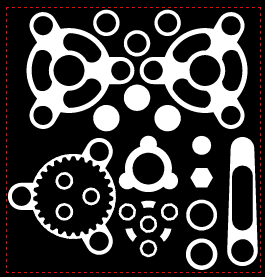
\includegraphics[keepaspectratio=true,width=0.5\textwidth]{advanced/svg_output/example_svg_slice.png}
\caption{Example de tranche SVG.}
\label{fig:example_svg_slice}
\end{figure}

\index{Menu!Slice to SVG...}
\index{Menu!Trancher au format SVG...}

Slic3r offre la possibilit\'e de produire une sortie SVG appropri\'e pour de telles imprimantes.  Au lieu d'utiliser le \texttt{Plater}, le processus commence par la s\'election de l'option \texttt{Slice to SVG...} du menu \texttt{File}.  Celui-ci demande le fichier source (STL, OBJ ou AMF), et lorsqu'il est s\'electionn\'e demande o\`u le fichier SVG de sortie doit \^etre enregistr\'e. Ensuite Slic3r d\'emarre et produit le fichier SVG.

Tenter de voir le fichier SVG dans un navigateur entra\^inera seulement l'affichage de la premi\`ere couche, et seules les \^iles n\'egatifs dans le mod\`ele (comme l'arri\`ere-plan du navigateur est g\'en\'eralement blanc).

\begin{figure}[H]
\centering
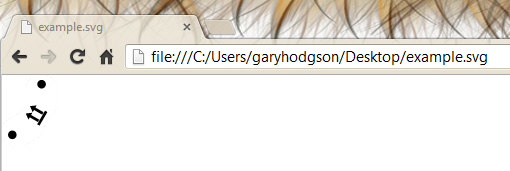
\includegraphics[keepaspectratio=true,width=0.75\textwidth]{advanced/svg_output/svg_direct_browser.png}
\caption{le fichier SVG vu dans un navigateur.}
\label{fig:svg_direct_browser}
\end{figure}

Pour cette raison, une petite application web a \'et\'e \'ecrite pour permettre de visualiser chaque tranche sur un fond noir\footnote{\url{http://garyhodgson.github.io/slic3rsvgviewer}}.  Acc\'edez \`a l'application et faites glisser le fichier SVG sur l'\'ecran pour le charger et l'afficher.

\begin{figure}[H]
\centering
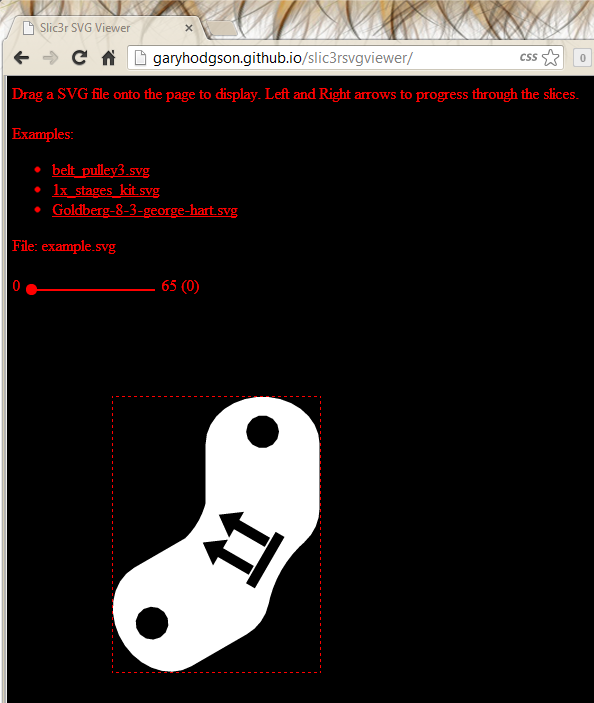
\includegraphics[keepaspectratio=true,width=0.75\textwidth]{advanced/svg_output/svg_slic3rsvg_viewer.png}
\caption{Slic3r SVG Viewer.}
\label{fig:svg_slic3rsvg_viewer}
\end{figure}

\subsection{Param\`etres SVG} % (fold)
\label{sub:svg_settings}

La majorit\'e des options dans Slic3r ne sont pas n\'ecessaires pour la g\'en\'eration SVG, cependant le param\`etre \texttt{Layer height} d\'eterminera le nombre de couches. Notez que Slic3r limite la hauteur de la couche pour qu'elle soit plus petite que le diam\`etre de la buse, donc cela peut \'egalement \^etre augmenter si l'on souhaite des couches plus hautes.

% subsection svg_settings (end)

\subsection{Imprimer \`a partir de fichiers SVG} % (fold)
\label{sub:printing_with_svg}

Alors que la sortie SVG peut \^etre utilis\'e pour une gamme d'imprimantes, l'exemple suivant montre comment le fichier, peut \^etre utilis\'e avec une imprimante r\'esine DLP. En utilisant une version modifi\'ee de Printrun \footnote{\url{http://garyhodgson.com/reprap/projectlayer}} le fichier SVG peut \^etre charg\'e directement et envoy\'e \`a un projecteur DLP. L'axe Z est contr\^ol\'ee par des commandes G-code envoy\'e par le composant printcore, ce qui signifie que l'\'electronique RepRap standard, tels que RAMPS, peuvent \^etre utilis\'es.


\begin{figure}[H]
\centering
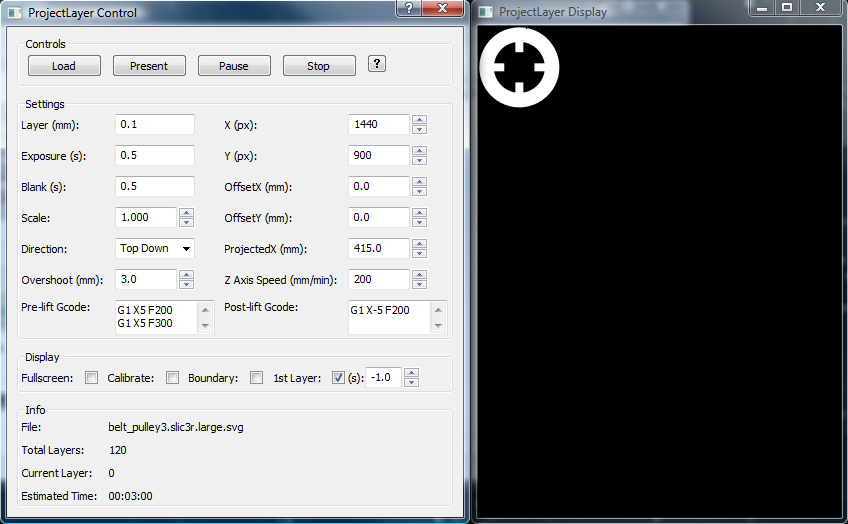
\includegraphics[keepaspectratio=true,width=0.75\textwidth]{advanced/svg_output/projectlayer.png}
\caption{Impression SVG avec Projectlayer.}
\label{fig:projectlayer}
\end{figure}


% subsection printing_with_svg (end)

% section svg_output (end)